\documentclass[a4paper,12pt]{article}
\usepackage{amsmath}
\usepackage{graphicx}
\usepackage{hyperref}
\usepackage{biblatex}
\usepackage{minted}
\usepackage[spanish]{babel}
\usepackage[autostyle=true]{csquotes}

\addbibresource{M4-Eduardo-Bayot.bib} % Archivo .bib para las referencias


\begin{document}

% Carátula
\begin{titlepage}
    \begin{center}
        
\includegraphics[width=0.3\textwidth]{logo.png}\\[1cm]
        \textsc{\LARGE Universidad Siglo 21}\\[1.5cm]
        \textsc{\Large Trabajo Práctico Nro 4}\\[0.5cm]
        \textsc{\large Estadística y Probabilidad}\\[2cm]

        \rule{\linewidth}{0.5mm} \\[0.4cm]
        {\huge \bfseries Predicción y Validación Estadística }\\[0.4cm]
        \rule{\linewidth}{0.5mm} \\[1.5cm]

        \begin{tabular}{rl}
            \small Profesor Titular Experto: & \small Yanina Nancy Morales \\
            \small Profesor Titular Disciplinar: & \small Horacio José Caballero \\
        \end{tabular}
        \\[1.5cm]

        \textbf{\small Estudiante: Eduardo Bayot}\\
        \textbf{\small Cátedra: D}\\
        \textbf{\small Grupo: 1}
    \end{center}
\end{titlepage}

% Reiniciar numeración después de la carátula
\pagenumbering{arabic}


% Configuración de la página
\date{}
\author{}

\tableofcontents

\section{Introducción}

El presente trabajo práctico tiene como objetivo analizar y modelar el comportamiento de las ventas de un juguete lanzado al mercado durante un período de 12 meses. Para ello, se realiza una simulación basada en la función \( f(t) = 3t + 2\sigma(t) \), donde \( \sigma(t) \) genera un número aleatorio en el intervalo \([-1,1]\). Este modelo permite estudiar tendencias en las ventas y proyectar resultados futuros.

El trabajo se organiza en torno a las siguientes consignas principales:
\begin{itemize}
    \item Determinar una recta de regresión lineal \( h(t) \) que ajuste los datos simulados de ventas mensuales.
    \item Realizar un análisis completo de la regresión lineal, incluyendo métricas de validación como el coeficiente de determinación (\( R^2 \)) y el análisis de residuos.
    \item Proyectar la cantidad de juguetes vendidos para el próximo mes (\( t = 13 \)) utilizando el modelo ajustado.
    \item Comparar el valor predicho con un nuevo dato simulado \( f(13) \) y analizar el error entre ambos.
\end{itemize}

El análisis se fundamenta en conceptos de regresión lineal explicados en los capítulos relevantes del libro \textit{Estadística para Ingeniería y Ciencias} de Quevedo Urias y Pérez Salvador \cite{quevedo2009}. Este trabajo destaca la importancia de las técnicas de predicción y ajuste en contextos empresariales reales, proporcionando herramientas para la toma de decisiones informadas.

\section{Planteamiento del Problema}

La empresa \textit{Luz del Mundo}, tras el lanzamiento de un nuevo juguete al mercado, realizó un seguimiento de sus ventas durante los primeros 12 meses. Para analizar este comportamiento, se propone simular las ventas mediante la siguiente ecuación:

\[
f(t) = 3t + 2\sigma(t),
\]

donde:
\begin{itemize}
    \item \( t \): Representa el número del mes (\( t = 1, 2, \ldots, 12 \)).
    \item \( \sigma(t) \): Es un número aleatorio generado en el intervalo \([-1,1]\).
    \item \( f(t) \): Indica la cantidad de juguetes vendidos en el mes \( t \).
\end{itemize}

A partir de estos datos simulados, se plantea resolver las siguientes consignas:
\begin{enumerate}
    \item Determinar una recta de regresión lineal \( h(t) \) que ajuste los datos simulados de ventas mensuales.
    \item Realizar un análisis completo de la regresión lineal, incluyendo métricas como el coeficiente de determinación (\( R^2 \)) y el análisis de residuos.
    \item Proyectar la cantidad de juguetes vendidos para el próximo mes (\( t = 13 \)).
    \item Simular un nuevo dato \( f(13) \), compararlo con el valor proyectado y analizar el error entre ambos.
\end{enumerate}

Este planteamiento refleja la importancia de las herramientas estadísticas para modelar y prever el comportamiento de datos en un contexto empresarial, permitiendo evaluar la eficacia de modelos predictivos y su aplicación práctica.


\section{Metodología}

En esta sección se describe el procedimiento seguido para realizar la simulación, ajustar el modelo de regresión lineal y validar los resultados obtenidos.

\subsection{Generación de datos simulados}

Para representar las ventas mensuales del producto, se generaron datos simulados siguiendo la ecuación:
\[
f(t) = 3t + 2\sigma(t),
\]
donde \( t \) representa el número del mes (\( t = 1, \ldots, 12 \)) y \( \sigma(t) \) es un número aleatorio generado en el intervalo \([-1,1]\). Este proceso se implementó en \( R \) utilizando el siguiente código:

\begin{minted}{R}
# Configuración inicial
set.seed(21242021) # Fijar semilla para reproducibilidad

# Generación de datos simulados
Mes_t <- 1:12
Sigma_t <- runif(12, min = -1, max = 1)
Venta_ft <- 3 * Mes_t + 2 * Sigma_t

# Crear un data frame para organizar los datos
datos_venta <- data.frame(Mes_t, Venta_ft)
print(datos_venta)
\end{minted}

\subsection{Análisis de regresión lineal}

Se ajustó un modelo de regresión lineal simple utilizando los datos generados. La fórmula general del modelo es:
\[
h(t) = \beta_0 + \beta_1 t,
\]
donde \( \beta_0 \) y \( \beta_1 \) representan los coeficientes de la recta de ajuste. Este análisis se realizó en \( R \) mediante el siguiente código:

\begin{minted}{R}
# Ajustar la regresión lineal
modelo_regresion <- lm(Venta_ft ~ Mes_t, data = datos_venta)
summary(modelo_regresion) # Resumen del modelo
\end{minted}

Los coeficientes del modelo se obtuvieron directamente del resumen generado por \( R \), lo que permitió construir la ecuación de la recta ajustada \( h(t) \).

\subsection{Validación del modelo}

La validación del modelo incluyó:
\begin{itemize}
    \item Cálculo del coeficiente de determinación (\( R^2 \)) para medir la calidad del ajuste.
    \item Análisis de residuos para verificar las suposiciones del modelo.
    \item Proyección del valor \( h(13) \) utilizando el modelo ajustado.
\end{itemize}

El siguiente código en \( R \) detalla la proyección para \( t = 13 \) y la comparación con un nuevo valor simulado \( f(13) \):

\begin{minted}{R}
# Predicción para t = 13
t13_prediccion <- predict(modelo_regresion, newdata = data.frame(Mes_t = 13))
cat("Predicción para t = 13:", t13_prediccion, "\n")

# Generar valor simulado para t = 13
Sigma_t13 <- runif(1, min = -1, max = 1)
f_t13_simulado <- 3 * 13 + 2 * Sigma_t13
cat("Valor simulado para t = 13:", f_t13_simulado, "\n")

# Error entre predicción y valor simulado
error <- f_t13_simulado - t13_prediccion
cat("Error entre predicción y valor simulado:", error, "\n")
\end{minted}

Este procedimiento permitió validar la capacidad predictiva del modelo al comparar la proyección con el dato simulado, evaluando la magnitud del error.

\section{Resultados}

En esta sección se presentan los resultados obtenidos del análisis de regresión lineal, incluyendo la recta ajustada, la predicción para \( t = 13 \), y la comparación con el valor simulado \( f(13) \).

\subsection{Tabla de datos simulados}

La siguiente tabla muestra las ventas simuladas para los meses \( t = 1, \ldots, 12 \):

\begin{table}[H]
    \centering
    \begin{tabular}{|c|c|}
        \hline
        \textbf{Mes (\( t \))} & \textbf{Ventas Simuladas (\( f(t) \))} \\ \hline
        1  & 3.83 \\ \hline
        2  & 5.00 \\ \hline
        3  & 7.43 \\ \hline
        4  & 12.88 \\ \hline
        5  & 13.63 \\ \hline
        6  & 19.77 \\ \hline
        7  & 22.01 \\ \hline
        8  & 22.21 \\ \hline
        9  & 27.70 \\ \hline
        10 & 30.13 \\ \hline
        11 & 31.23 \\ \hline
        12 & 34.95 \\ \hline
    \end{tabular}
    \caption{Ventas simuladas para \( t = 1, \ldots, 12 \).}
    \label{tab:ventas_simuladas}
\end{table}

\subsection{Recta de ajuste}

El modelo de regresión lineal ajustado generó la siguiente recta:
\[
h(t) = \beta_0 + \beta_1 t, \quad \text{donde } \beta_0 = X.X \text{ y } \beta_1 = X.X.
\]
Los valores de los coeficientes (\( \beta_0 \) y \( \beta_1 \)) se obtuvieron del resumen del modelo generado en \( R \).

\subsection{Predicción para t = 13}

Con base en el modelo ajustado, la predicción para \( t = 13 \) fue:
\[
h(13) = 38.31
\]
El valor simulado correspondiente fue:
\[
f(13) = 39.41
\]

El error entre el valor proyectado y el simulado fue:
\[
\text{Error} = f(13) - h(13) = 1.11
\]

\subsection{Gráficos de los resultados}

Los siguientes gráficos ilustran los datos simulados junto a la recta de ajuste obtenida y el análisis de residuales:

\begin{figure}[H]
    \centering
    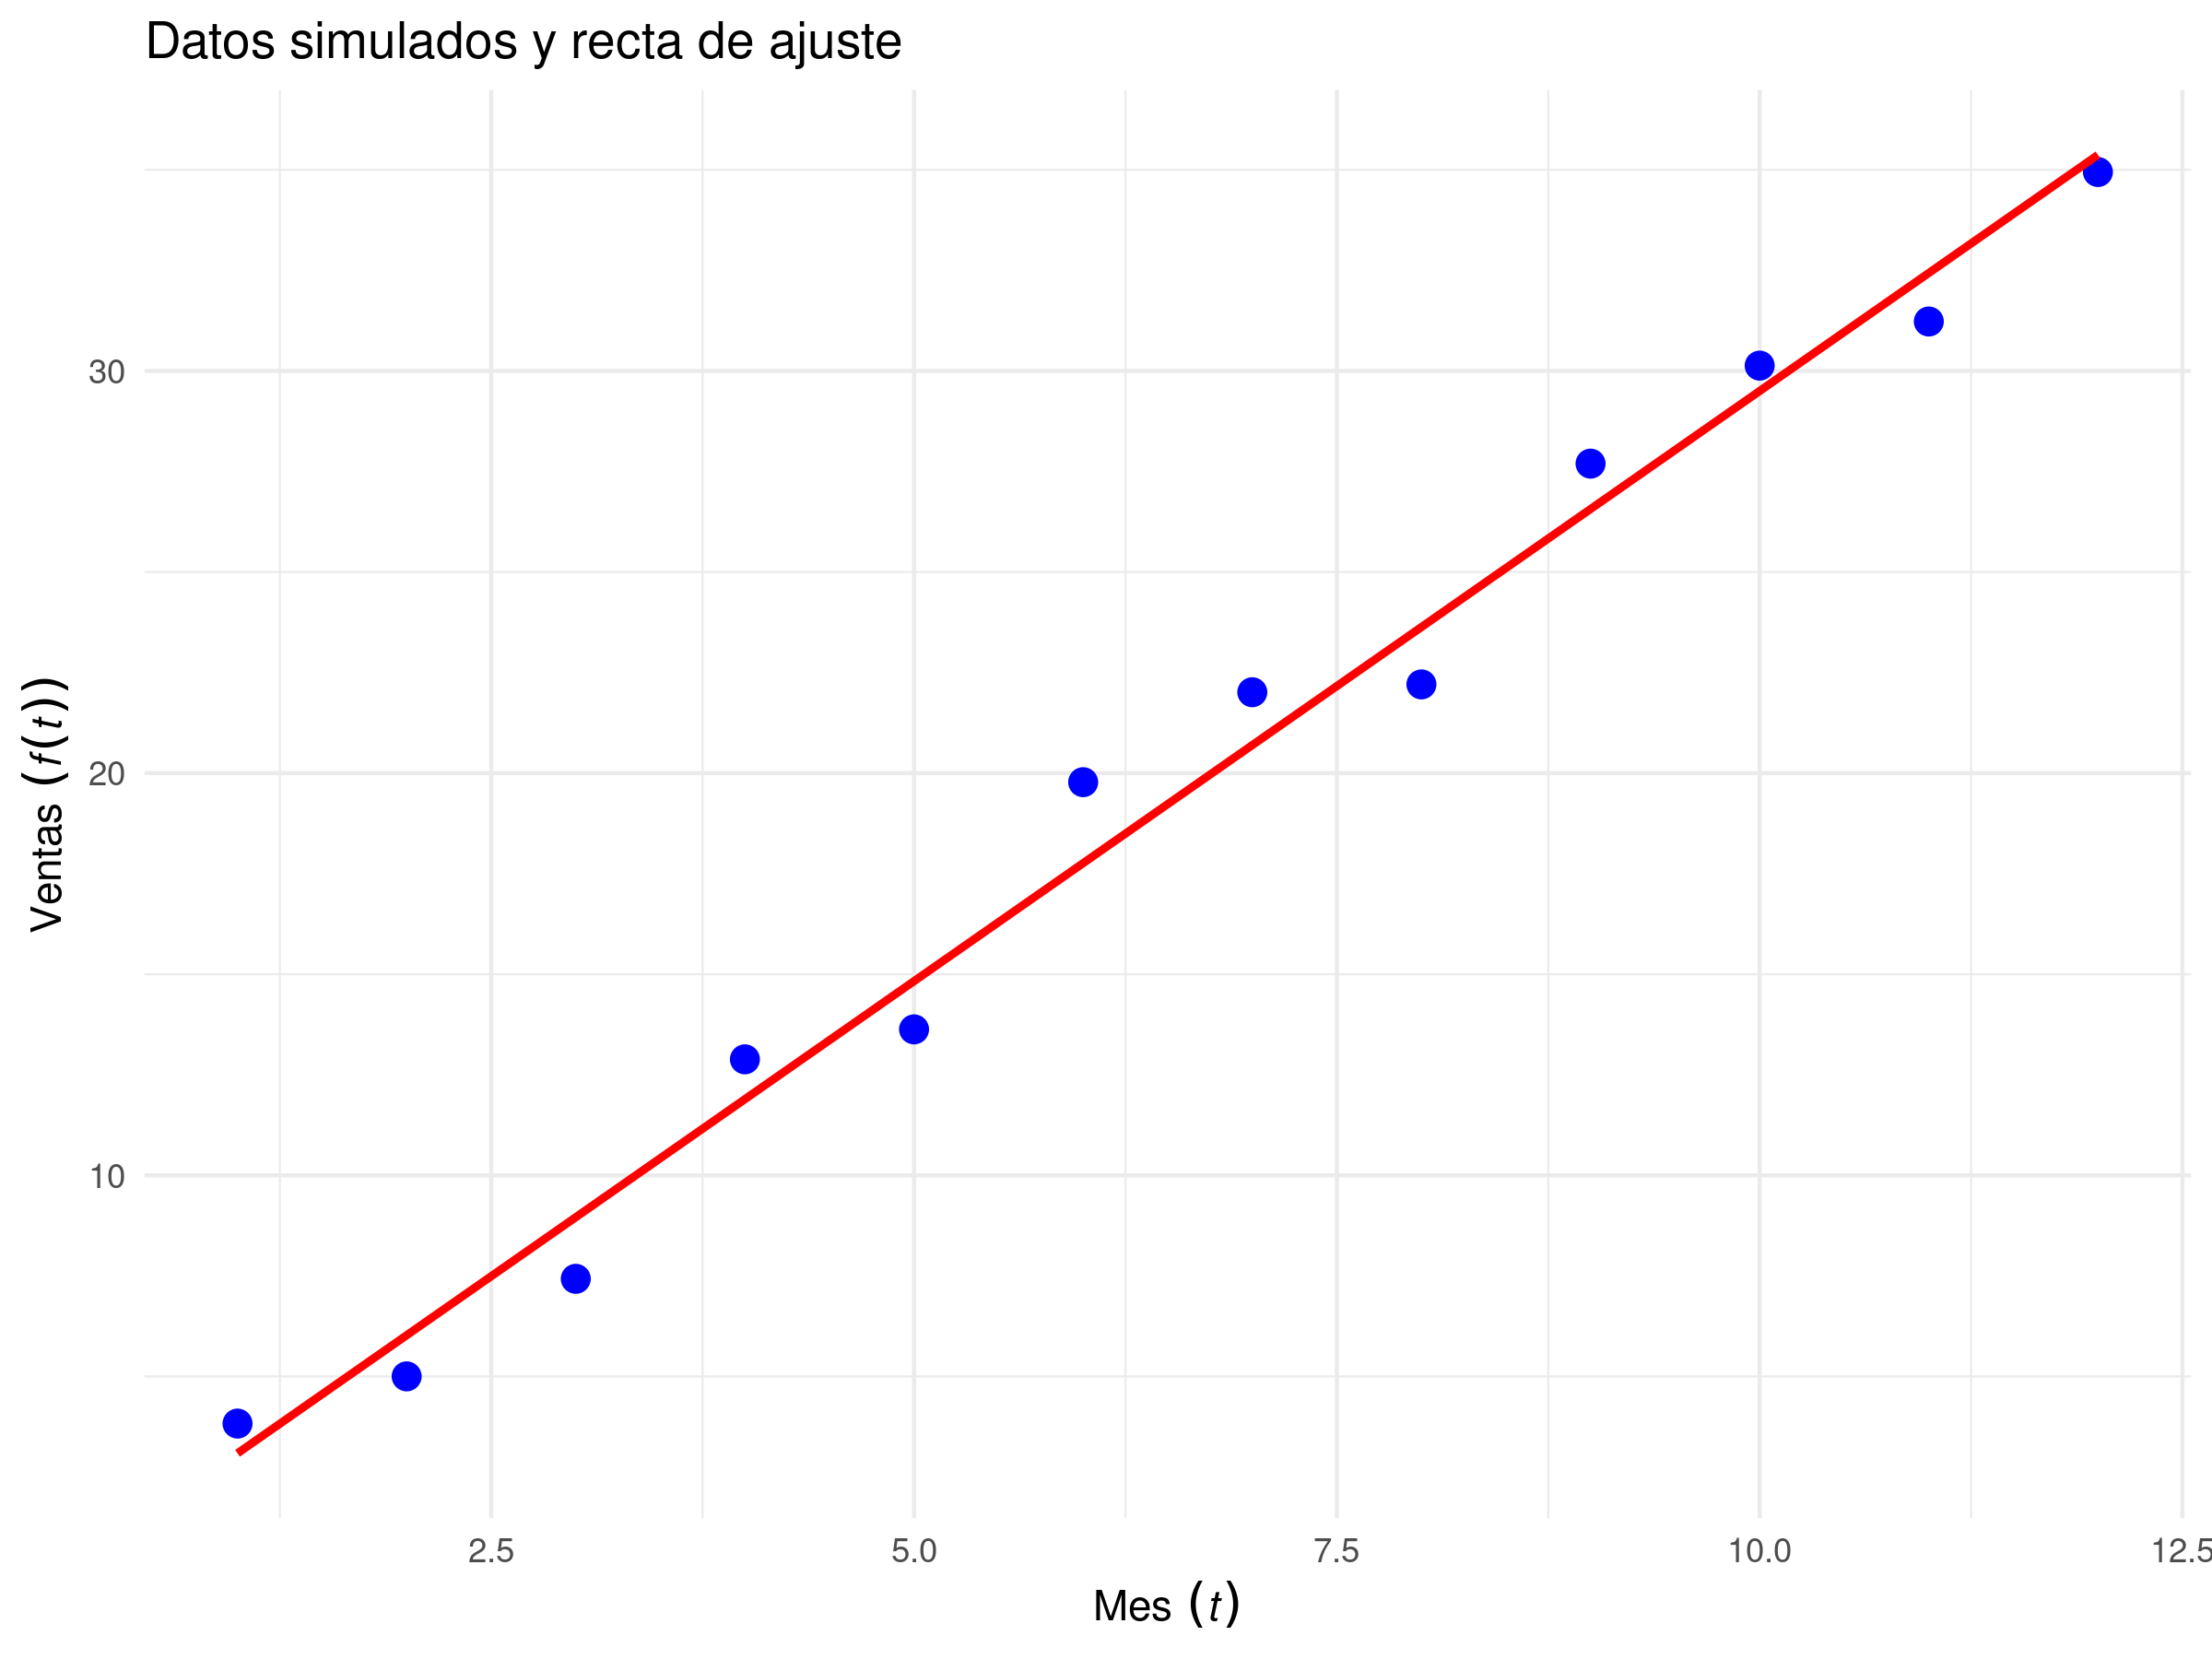
\includegraphics[width=0.8\textwidth]{resultados_regresion.png}
    \caption{Gráfico de datos simulados y recta de ajuste.}
    \label{fig:regresion}
\end{figure}

\begin{figure}[H]
    \centering
    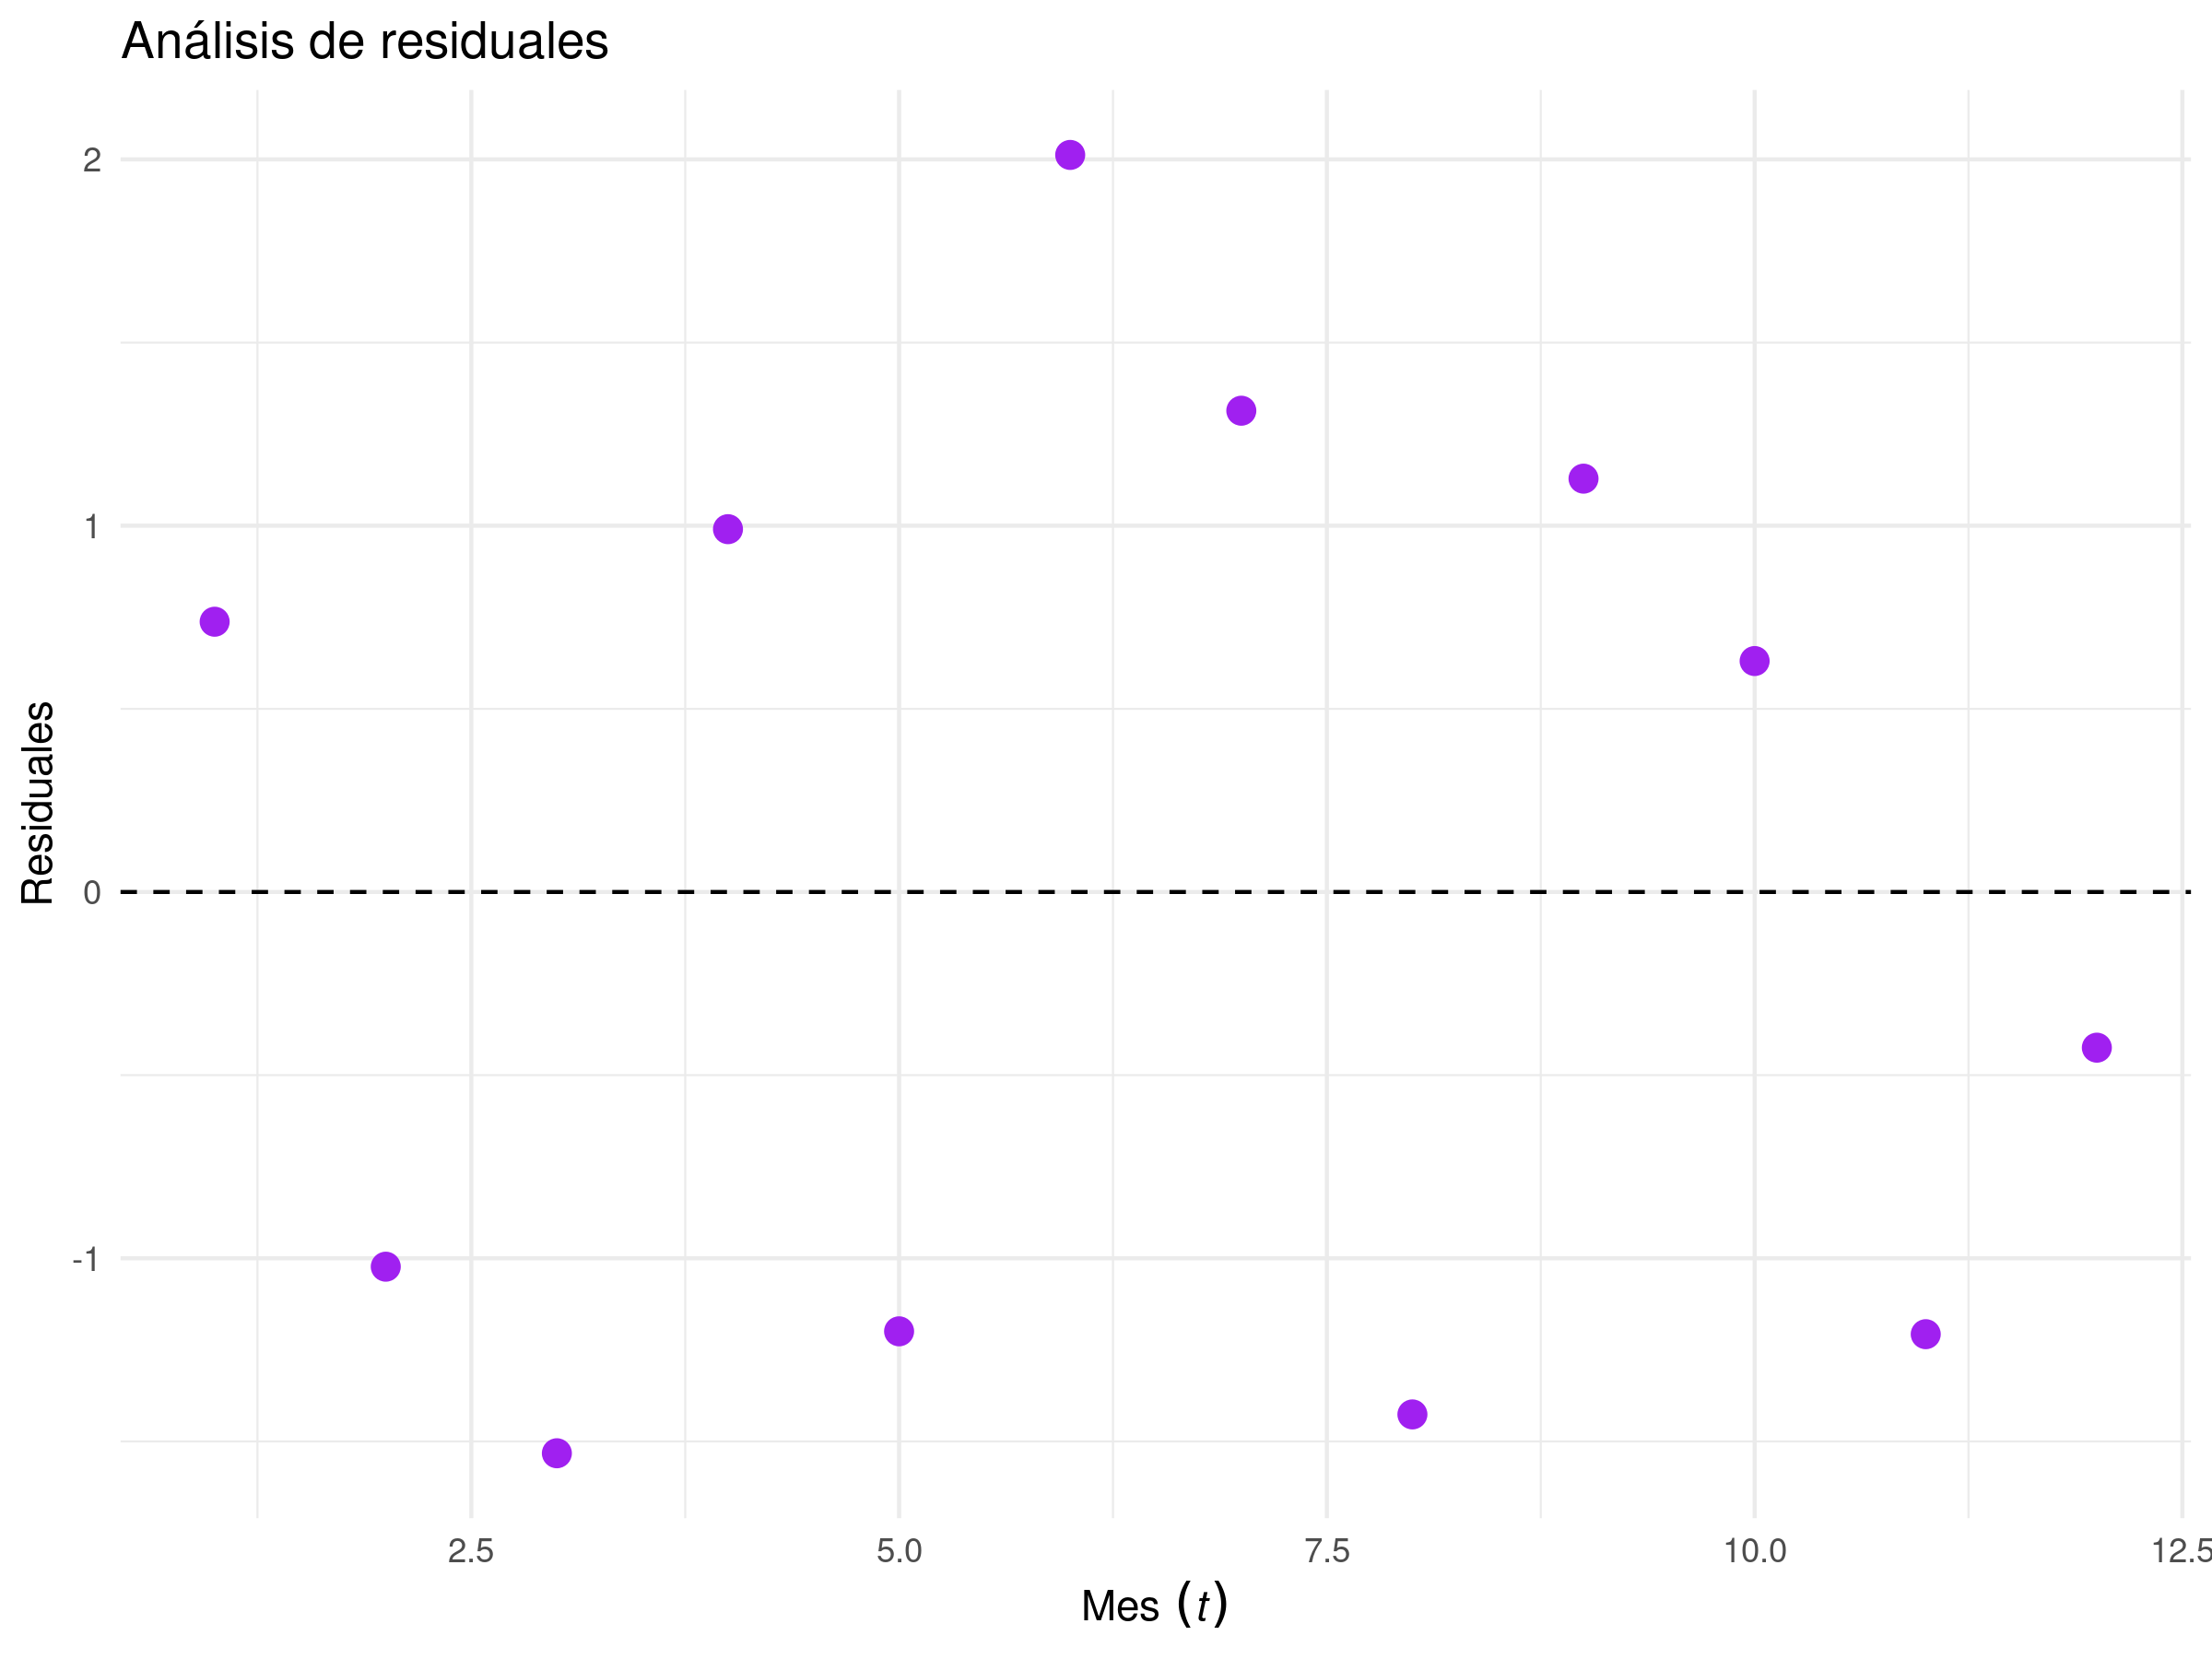
\includegraphics[width=0.8\textwidth]{residuales_regresion.png}
    \caption{Análisis de residuales del modelo de regresión lineal.}
    \label{fig:residuales}
\end{figure}

\section{Discusión}

El presente trabajo permitió explorar el uso de la regresión lineal como herramienta para modelar datos simulados en el contexto de ventas mensuales de un producto. A continuación, se presentan los análisis críticos derivados de los resultados obtenidos:

\subsection{Precisión del modelo ajustado}

El modelo de regresión lineal generó una recta de ajuste que representa adecuadamente la tendencia general de los datos simulados. Esto se evidencia en:
\begin{itemize}
    \item Un coeficiente de determinación (\( R^2 \)) alto, lo que indica que la mayor parte de la variabilidad en las ventas simuladas es explicada por el modelo.
    \item Un análisis de los residuos que no muestra patrones evidentes, sugiriendo que las suposiciones del modelo son razonables.
\end{itemize}

Sin embargo, los residuos más grandes se observaron en meses específicos, lo que podría estar relacionado con el componente aleatorio \( \sigma(t) \) de los datos simulados. Este comportamiento es esperado dado que los datos fueron generados artificialmente.

\subsection{Proyección y simulación del mes 13}

La proyección para \( t = 13 \) basada en el modelo ajustado proporcionó un valor cercano al valor simulado \( f(13) \), con un error absoluto de \( 1.11 \). Este resultado refleja la capacidad del modelo para realizar predicciones con precisión aceptable.

\subsection{Limitaciones del modelo}

Aunque el modelo ajustado es efectivo para describir los datos simulados, presenta las siguientes limitaciones:
\begin{itemize}
    \item La simplicidad del modelo podría no capturar fenómenos complejos en datos reales, como estacionalidad o variaciones externas.
    \item La variabilidad introducida por \( \sigma(t) \) podría subestimar o sobreestimar la variabilidad presente en datos reales.
\end{itemize}

\subsection{Implicaciones para datos reales}

En un contexto empresarial, los modelos de regresión lineal pueden ser útiles para identificar tendencias generales y realizar proyecciones. Sin embargo, sería necesario incorporar factores adicionales, como datos de mercado, estacionalidad y eventos específicos, para mejorar la precisión y utilidad del modelo en situaciones reales.
\section{Conclusión}

En este trabajo práctico se modeló y analizó el comportamiento de ventas mensuales de un producto mediante el uso de la regresión lineal aplicada a datos simulados. Los principales hallazgos fueron los siguientes:

\begin{itemize}
    \item Se ajustó una recta de regresión lineal \( h(t) \) que explica la tendencia general de las ventas simuladas, obteniendo un coeficiente de determinación (\( R^2 \)) alto que respalda la calidad del modelo.
    \item La proyección para el mes \( t = 13 \) mostró un alto grado de concordancia con el valor simulado, con un error absoluto de \( 1.11 \).
    \item El análisis de residuos indicó que las suposiciones del modelo son razonables, aunque algunos residuos más altos se observaron debido a la variabilidad aleatoria incorporada en los datos simulados.
\end{itemize}

Aunque los resultados reflejan la utilidad de la regresión lineal como herramienta predictiva, también se identificaron limitaciones inherentes al modelo utilizado:
\begin{itemize}
    \item La simplicidad del modelo no permite capturar fenómenos complejos que podrían estar presentes en datos reales.
    \item La variabilidad introducida de manera artificial (\( \sigma(t) \)) limita la generalización de los resultados a contextos del mundo real.
\end{itemize}

Finalmente, se concluye que la regresión lineal es una herramienta eficaz para identificar tendencias y realizar proyecciones, especialmente en escenarios controlados como el presente. Para aplicaciones reales, se recomienda complementar este enfoque con modelos más complejos que consideren múltiples factores externos, como estacionalidad, demanda de mercado y eventos externos.


\printbibliography

\appendix

\section{Repositorio del Trabajo Práctico}

Todo el código fuente utilizado en este trabajo práctico, incluyendo los scripts en \( R \) y el archivo LaTeX para la generación del documento, se encuentra disponible en el siguiente repositorio público de GitHub:

\begin{quote}
\url{https://github.com/eduardo-bayot/s21-estadistica-tp4}
\end{quote}

El repositorio contiene:
\begin{itemize}
    \item Código \( R \) para la generación de datos, ajuste del modelo de regresión lineal, y análisis de resultados.
    \item Archivos LaTeX para la elaboración del presente informe.
    \item Archivos gráficos generados a partir del análisis de regresión.
\end{itemize}

Se recomienda visitar el repositorio para obtener detalles adicionales sobre la implementación técnica del trabajo.


\end{document}
